\subsubsection{Testing the MQ6 gas sensor}
\par Next, we wanted to test this sensor independently. To do this we first started off with reading the data-sheet to find out the appropriate voltage input and pin layout. We found out that it operates at 5 volts with a minimum of 0 volts. We supplied 5 volts from the power supply to our breadboard and we used an LED to our output pin to see if it detects any gas. 
\begin{figure}[h!]
	\centering
	\begin{subfigure}[t]{0.45\textwidth}
		\centering
		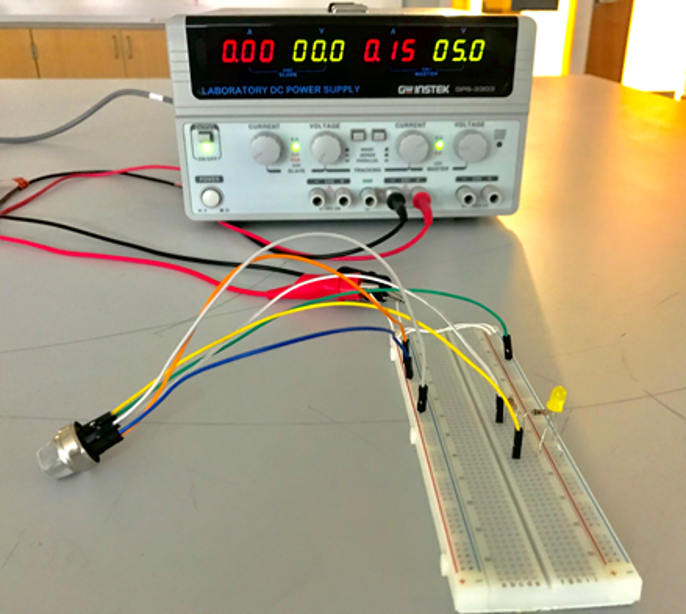
\includegraphics[height=1.5in]{mq6Test.png}
		\caption{LED on via pin 18}
	\end{subfigure}
	\begin{subfigure}[t]{0.45\textwidth}
		\centering
		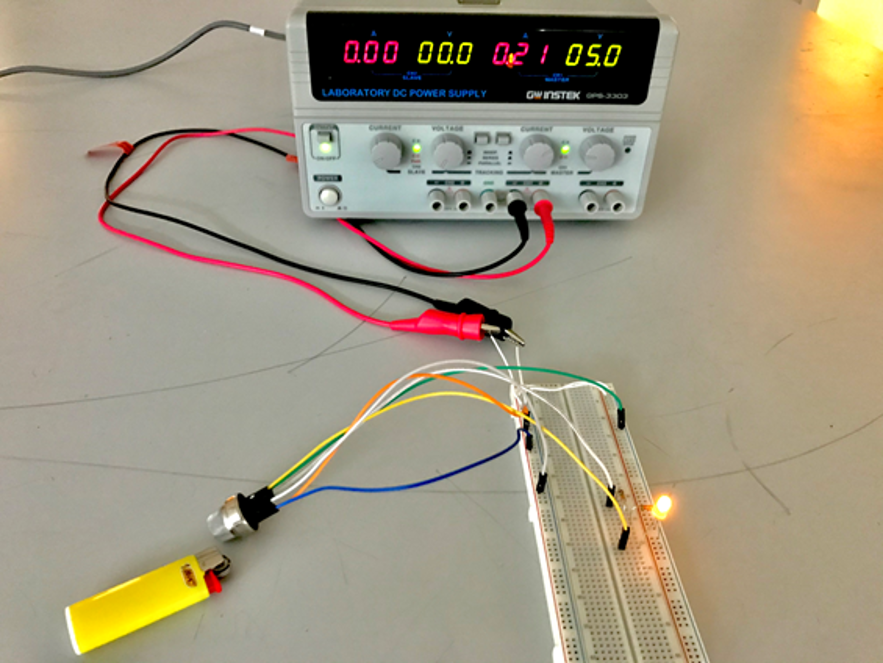
\includegraphics[height=1.5in]{mq6TestOn.png}
		\caption{LED off via pin 18}
	\end{subfigure}
	\caption{Simple LED activation over 802.15.4 (2)}
\end{figure}
\par Properly connected, the gas sensor produced quantifiable results. Using a common butane lighter, we tested the sensors ability to detect ambient gases. The LED was able to indicate the presence of LPG, thus we now know our gas sensing components are functional.
\par Since the XBee modules analog to digital converter requires an input in the range of 1.2 volts, we must reduce the 5 volt output of the gas sensor down to this level to be quantified and processed. To do this a simple voltage divider was designed (1). With voltages constant and one resistor value constant we only need to solve for one unknown (2).
\begin{equation}
V\textsubscript{out}=\frac{R1}{R1+R2}*V\textsubscript{in}
\end{equation}
Solving for R1: \\
\begin{equation}
1.2 = \frac{5100}{R1+5100}*5
\end{equation}
\[R1 = 16150 \Omega\]

% Testing the PIR Motion sensor
\subsubsection{Testing the PIR Motion Sensor}
\par The Parallax sensor allows us to choose between two set trip duration options, either an approximate time of 2 seconds or 5 seconds. This means that when the sensor is triggered it will hold its output high for the selected option. This setting is changed with the manual moving of a jumper that connects a center pin with a second pin either on its left or right. In essence this is a crude switch. To yield as flexible a system as possible, a small DIP switch has been designed to toggle this setting. This allows the user to decide between a "Shorter" or "Longer" setting depending on which is best suited to their operating environment. This would be set to the "Shorter" option by default. 
\par In initial testing of the sensor, the output received at the XBee itself was subject to some instability. This was solved by adding an RC filter between the digital input of the XBee and the output of the sensor module. This eliminated a DC component that would sometimes be present in the signal. 

 


\subsubsection{Testing Raspberry Pi \& Camera}
\paragraph{Camera difficulties} Camera Component sends a camera control callback error and does not take and save pictures anymore. The OS of the raspberry pi has been reset and redownloaded to the raspberry pi. There is a visible trigger to the camera activating when using the Pi NOIR camera board. There is a red light on the board of the camera that signifies when it is turned on or activated. The camera when activated through the command window will sometimes create the file but have no data inside of it. Upon receiving this error it seems to slow down the raspberry pi board significantly that it requires a restart. The raspberry pi has been test with three different camera modules and all of them give back the same callback control error.  Raspberry Pi has configuration settings to activate and recognize when a camera is connected, however the issues may seem to arise with a faulty port on the raspberry pi itself.
\begin{figure}[h]
	\begin{lstlisting}
	mmal: Received unexpected camera control callback event, 0x4f525245
	\end{lstlisting}
	\label{fig:camErr}
	\caption{Error from camera module}
\end{figure}
\par When attempting to switch to audio recording instead of using the camera the only devices available were 3.5mm jack from a headset with built in microphone. The assumption was to connect to the audio jack output of the raspberry pi, and record and listen through the headset itself. However, this is impossible due to the specifications of the raspberry pi the audio jack is meant for output only. The only way to record audio was using a 